\section{Methodology}

Our analysis considers a representative set of AI agents and benchmarking workloads, covering diverse agent workflows and agentic task characteristics.

\begin{scriptsize}
\begin{table}[t]
\centering
\caption{Comparison of AI agents.}
\scriptsize
\begin{tabular}{cccccc}
\hline
\textbf{Agent} & \textbf{Reasoning} & \makecell[c]{\textbf{Tool}\\ \textbf{Use}} & \textbf{Reflection} & \makecell[c]{\textbf{Tree}\\ \textbf{Search}} & \makecell[c]{\textbf{Structured}\\ \textbf{Planning}} \\ \hline\hline
\textbf{CoT}~\cite{cot} & O & X & X & X & X \\ 
\textbf{ReAct}~\cite{react} & O & O & X & X & X \\ 
\textbf{Reflexion}~\cite{reflexion} & O & O & O & X & X \\ 
\textbf{LATS}~\cite{lats} & O & O & O & O & X \\ 
\textbf{LLMCompiler}~\cite{llmcompiler} & O & O & O & X & O \\ \hline
\end{tabular}
\label{tab:agents}
\end{table}
\end{scriptsize}

\begin{figure}[t!] \centering
\captionsetup[subfloat]{captionskip=0.1em}
\subfloat[CoT]{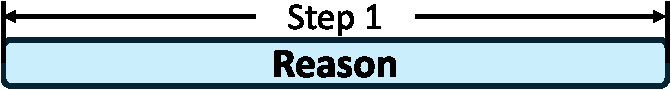
\includegraphics[width=0.19\textwidth]{./fig/timeline_cot}}\\
\subfloat[ReAct]{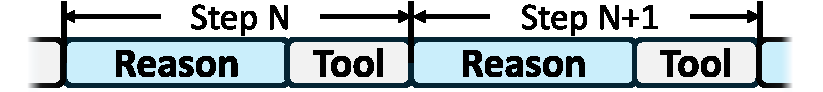
\includegraphics[width=0.24\textwidth]{./fig/timeline_react}}\\
\subfloat[Reflexion]{
\includegraphics[width=0.32\textwidth]{./fig/timeline_reflexion}}\\
\subfloat[LATS]{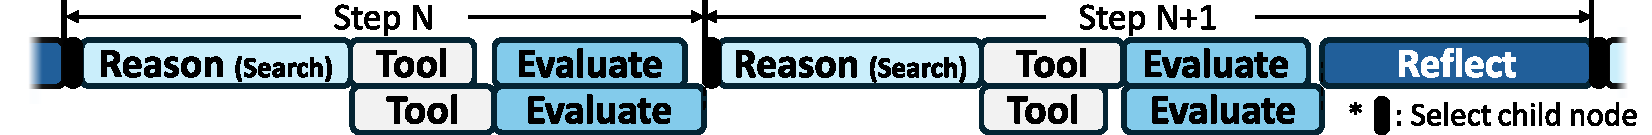
\includegraphics[width=0.48\textwidth]{./fig/timeline_lats}}\\
\subfloat[LLMCompiler]{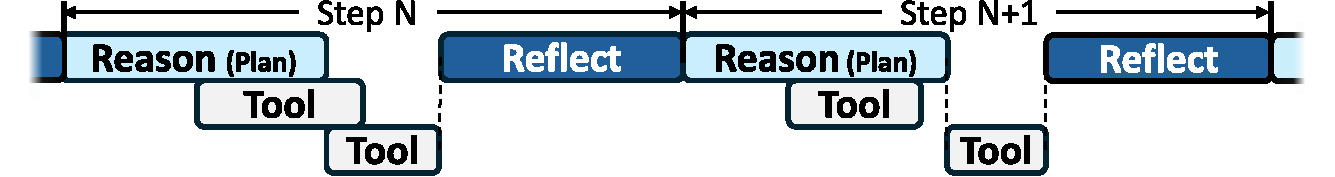
\includegraphics[width=0.39\textwidth]{./fig/timeline_llmcompiler}}
\label{fig:agent_timeline_llmcompiler}
\\
\caption{Execution timeline of each AI agent.}
\label{fig:agent_timeline}
\vspace{-0.8em}
\end{figure}


\textbf{AI agent workflows.} 
We investigate five representative agents: Chain-of-Thought (CoT)~\cite{cot}, ReAct~\cite{react}, Reflexion~\cite{reflexion}, Language Agent Tree Search (LATS)~\cite{lats}, and LLMCompiler~\cite{llmcompiler}. These agents were selected to cover a wide range of reasoning strategies, tool integrations, and planning mechanisms. Table \ref{tab:agents} summarizes the presence or absence of five key capabilities across each agent.

\begin{itemize}[leftmargin=1em]
    \item \textbf{Reasoning.} All agents considered in this study employ a reasoning mechanism. Among them, CoT operates purely through internal reasoning without the use of any external tool (\fig{fig:agent_timeline}(a)). As a baseline for comparison, CoT-style static reasoning approaches are considered within the broader definition of AI agents, despite their lack of external interactions with tools.
    
    \item \textbf{Tool use.} Tool use differentiates purely language-based agents from those capable of interacting with the external environment. This functionality enables agents to access real-time data or perform non-linguistic operations.

    \item \textbf{Reflection.} Reflection allows agents to evaluate past decisions and revise strategies accordingly. Reflective agents effectively manage \emph{long-term memory} by abstracting past trajectories into reflections. While ReAct agents simply repeat reasoning and tool usage (\fig{fig:agent_timeline}(b)), Reflexion, the most fundamental reflective agent, enhances adaptability by periodically incorporating self-evaluation and refinement through reflection (\fig{fig:agent_timeline}(c)).

    \item \textbf{Tree search.} LATS (\fig{fig:agent_timeline}(d)) leverages Monte Carlo Tree Search~\cite{mcts} to simulate multiple branches of reasoning and action, allowing the agent to evaluate different candidate paths before making a decision. By simulating multiple possible future paths, the agent can make more informed decisions and select optimal action sequences.

    \item \textbf{Structured planning.} LLMCompiler incorporates a structured multi-step planning and streaming for asynchronous task execution to minimize latency. During the planning phase, LLMCompiler analyzes task dependencies and constructs a DAG that organizes future tool calls into an execution plan. This enables multiple dependent tool calls to be generated within a single LLM invocation. As the plan is constructed, intermediate tool calls are streamed to the execution stage, allowing the scheduler to overlap planning and tool calls via asynchronous execution. Together, these features can help reduce repeated reasoning and lower end-to-end latency (\fig{fig:agent_timeline}(e)).
\end{itemize}

In general, we utilized the official open-source implementations provided by the original authors of these agent workflows~\cite{react_github,reflexion_github,lats_github,llmcompiler_github}. Each AI agent is adapted to support our evaluation framework and benchmarks. For LATS, we further optimized its implementation to support concurrent LLM inference and parallel tool invocation because the original version~\cite{lats_github} executes these operations sequentially, aggravating end-to-end latency.

\begin{scriptsize}
\begin{table}[t]
\centering
\caption{Description of benchmarks.}
\scriptsize
\begin{tabular}{ccc}
\hline
\textbf{Benchmark} & \textbf{Property} & \textbf{Description} \\ \hline\hline
\multirow{3}{*}{\textbf{HotpotQA}~\cite{hotpotqa}} 
    & \textbf{Task} & Multi-hop question answering \\ \cline{2-3}
    & \textbf{Tool} & Wikipedia APIs (search, lookup keywords)\\ \cline{2-3}
    & \textbf{Agent} & CoT, ReAct, Reflexion, LATS, LLMCompiler \\ \hline
\multirow{3}{*}{\textbf{WebShop}~\cite{webshop}} 
    & \textbf{Task} & Online shopping \\ \cline{2-3}
    & \textbf{Tool} & Interactive web navigation (search, click) \\ \cline{2-3}
    & \textbf{Agent} & ReAct, Reflexion, LATS, LLMCompiler \\ \hline
\multirow{3}{*}{\textbf{MATH}~\cite{math}} 
    & \textbf{Task} & Math problem solving \\ \cline{2-3}
    & \textbf{Tool} & Wolfram Alpha API, Python-based calculator \\ \cline{2-3}
    & \textbf{Agent} & CoT, ReAct, Reflexion, LATS \\ \hline
\multirow{3}{*}{\textbf{HumanEval}~\cite{humaneval}} 
    & \textbf{Task} & Programming \\ \cline{2-3}
    & \textbf{Tool} & Executing self-generated test code \\ \cline{2-3}
    & \textbf{Agent} & CoT, ReAct, Reflexion, LATS \\ \hline
\end{tabular}
\label{tab:benchmarks}
\end{table}
\end{scriptsize}


\textbf{Benchmarks.}
We select four popular benchmarks representative of various downstream agentic tasks, whose descriptions are summarized in \tab{tab:benchmarks}. 
HotpotQA~\cite{hotpotqa} is a question-answering benchmark that assesses the agent's ability to accurately retrieve relevant evidence to answer multi-hop knowledge-intensive questions. We provide the Wikipedia APIs~\cite{wikipedia_api} as tools to solve these questions.
WebShop~\cite{webshop} is a web-shopping benchmark where agents find the best-fit item that meets the given conditions. The agent is given web navigation tools to browse WebShop.
MATH~\cite{math} is a benchmark suite of mathematics problems across various domains. Agents are equipped with access to the Wolfram Alpha API~\cite{wolfram_alpha_api} for solving complex equations, as well as a Python-based calculator for simple numerical computations.
HumanEval~\cite{humaneval} evaluates the programming capability of agents. In our setup, agents are equipped with a Python execution tool that allows them to validate the generated solutions by executing self-written test code.
In addition to these agentic benchmarks, we utilize a \emph{non-agentic} dataset, which is the ShareGPT dataset~\cite{sharegpt}, to model conventional chatbot-like LLMs, characterized by single-turn LLM inference without iterative interactions with the external environments. ShareGPT contains a collection of real conversations between users and ChatGPT~\cite{chatgpt}, capturing standard interactive dialogue scenarios.


It is worth pointing out that some ``AI agent vs. benchmark'' pairs are omitted if the agent is not suitable for solving the target task. For example, CoT is excluded from WebShop since it cannot interact with the shopping webpage. Similarly, LLMCompiler is omitted from MATH and HumanEval, as its DAG-style planning is not well-suited for problems that require sequential, step-by-step reasoning and tool usage.

\textbf{LLM backend.}
We employed the OpenAI-compatible vLLM (version 0.6.6) server as the LLM serving infrastructure, integrated with PyTorch 2.6 and CUDA 12.8. We enabled \emph{prefix caching}~\cite{vllm}, which reduces redundant computation by reusing previously computed attention states (i.e., \emph{Key-Value cache (KV cache)}) for shared input prefixes across LLM requests. Unless explicitly stated otherwise, all experimental results are obtained with prefix caching enabled. We use Llama-3.1-8B-Instruct~\cite{llama_3.1_8b_instruct} as the default backend LLM. However, to discuss the impact of model size on cost and accuracy, we also use Llama-3.1-70B-Instruct~\cite{llama_3.1_70b_instruct} in \sect{sect:char_implication}.

\textbf{Hardware.}
Experiments were conducted on Google Cloud Platform (GCP). For the 8B model, we used the \texttt{a2-highgpu-1g} instance type with 12 vCPUs (6 physical cores), 85GB memory, and a single NVIDIA A100 40GB GPU\footnote{
In this work, we use GPU-based serving systems for our analysis because they are the de facto standard for large-scale LLM serving. Our characterization methodology and findings are architecture-agnostic and directly transferable to other accelerator platforms like Google TPUs. As detailed in the rest of this paper, key insights such as the impact of agentic control-flow serialization, long-context KV cache pressure, and idle-period underutilization are inherent to the workload characteristics of dynamic reasoning, not to any GPU/TPU-specific microarchitecture. Thus, the system-level implications we identify remain equally relevant to other AI inference accelerators, providing a foundation for future cross-architecture analyses.}. For the 70B model, we used the \texttt{a2-highgpu-8g} instance type with 96 vCPUs (48 physical cores), 680GB memory, and 8 NVIDIA A100 40GB GPUs.